\documentclass{article}
\usepackage[utf8]{inputenc}
\setlength{\oddsidemargin}{0.25 in}
\setlength{\evensidemargin}{-0.25 in}
\setlength{\topmargin}{-0.6 in}
\setlength{\textwidth}{6.5 in}
\setlength{\textheight}{8.5 in}
\setlength{\headsep}{0.75 in}
\setlength{\parindent}{0 in}
\setlength{\parskip}{0.1 in}

\newtheorem{theorem}{Theorem}
\newtheorem{corollary}{Corollary}
\newtheorem{proposition}{Proposition}
\newtheorem*{remark}{Remark}
\theoremstyle{definition}
\newtheorem{example}{Example}
\newtheorem{definition}{Definition}

\newcommand{\lecture}[4]{
   \pagestyle{myheadings}
   \thispagestyle{plain}
   \newpage
%   \setcounter{lecnum}{#1}
   \setcounter{page}{1}
   \noindent
   \begin{center}
   \framebox{
      \vbox{\vspace{2mm}
    \hbox to 6.58in { {\bf CSC~565: Graph Theory
                        \hfill North Carolina State University} }
    \hbox to 6.58in { {\bf Fall 2019
                        \hfill Computer Science} }
       \vspace{4mm}
       \hbox to 6.28in { {\Large \hfill Lecture #1: #2  \hfill} }
       \vspace{2mm}
       \hbox to 6.28in { {\it Lecturer: {\it Don Sheehy {\tt <drsheehy@ncsu.edu>}} \hfill Scribe: #4} }
      \vspace{2mm}}
   }
   \end{center}
   \markboth{Lecture #1: #2}{Lecture #1: #2}
   \vspace*{4mm}
}

\usepackage{amsfonts}
\usepackage{amsmath,latexsym,amsbsy,amssymb}
\usepackage{graphicx}
\usepackage{geometry}  
\usepackage{paracol}
\usepackage{enumitem}
\usepackage{tcolorbox}

%\newtheorem{theorem}{Theorem}
\newtheorem{lemma}{Lemma}
\newtheorem{proposition}{Proposition}
\newtheorem{scolium}{Scolium}   %% And a not so common one.
\newtheorem{definition}{Definition}
\newenvironment{proof}{{\sc Proof:}}{~\hfill QED}
\newenvironment{AMS}{}{}
\newenvironment{keywords}{}{}


%\title{Lecture 15}
%\date{October 14 2019}
%\author{ Carl Klier, Nuhal Ravindra, Shahil Shah, Erica Swain  }
\begin{document}

\lecture{15}{Oct 14, 2019}{Don Sheehy}{Carl Klier, Nuhal Ravindra, Shahil Shah, Erica Swain }

\section{Review}
Last class we proved a specific case of Fary's Theorem, which says:
\begin{theorem}[Fary]
If a graph $G$ is planar, then there exists a linear embedding of $G$.
\end{theorem}
Additionally, in the last class we saw that if a planar graph is 2-connected, then its faces are bounded by cycles and a planar graph is 3-connected if and only if its faces are nonseparating induced cycles. \\
\section{Embedding in $\mathbb{R}^2$}
We have been studying embeddings of  the geometric realizations of graphs, i.e functions \\$f:geom(G)\to \mathbb{R}^2$.
\\\\ Now we want to geometrically understand why we can have any face of our graph G be the outer face in our embedding, by first understanding what an outer face is.
\\\\ First, notice that if we compose $f$ with a homeomorphism $g:\mathbb{R}^2\to \mathbb{R}^2$, $g\circ f: geom(G)\to \mathbb{R}^2$ is also an embedding. But instead, if we remove a small circle in the face of the graph we want to be the outer face and have a homeomorphism $h: \mathbb{R}^2\backslash$hole$\to \mathbb{R}^2\backslash$hole, then is $f\circ h$ an embedding?
\\\\
The answer is Yes!
\\\\
We get an embedding by the process called inverting the circle. This idea comes from the fact that $\mathbb{R} \cong S^1 \backslash P$ where $S^1$ is a circle and $P$ is a point and $\mathbb{R}^2 \cong S^2 \backslash P$ where $S^2$ is a sphere and $P$ is again a point. We can find the explicit map for the circle as well as the sphere as follows. If we take the unit circle and place it on a line, we draw a line through the north pole of the circle to any point on the line. This intersects the circle in some place, and this is where the point on the line is mapped to. For any point on the line no matter how far away it is, there is always a line through the north pole that intersects the circle and goes to that point. However, there is not actually a point on the line that  maps to the north pole. If there was, you would have to think of it as infinitely far away in both directions. Then we call this point $P$ the point at infinity, because it is "gluing" the two ends of the infinite line together. We can do the same thing to get an isomorphism between $\mathbb{R}^2$ and $S^2 \backslash P$. This homeomorphism helps us understand what it means to be the outer face, i.e. it is the back face on the rest of the sphere. \\
\centerline{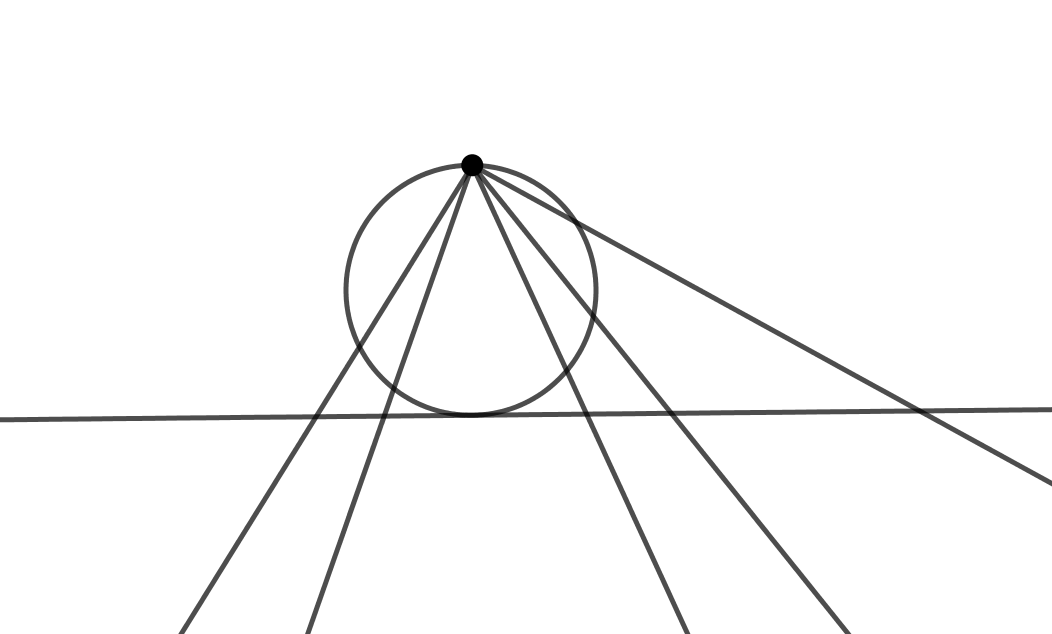
\includegraphics[width=2.25in]{Images/Homeomorphism.png}}
\\\\
If there is some face that would cover that patch of the sphere on top like in the drawing below, that would get mapped down to be the outer face.
\\\\
\centerline{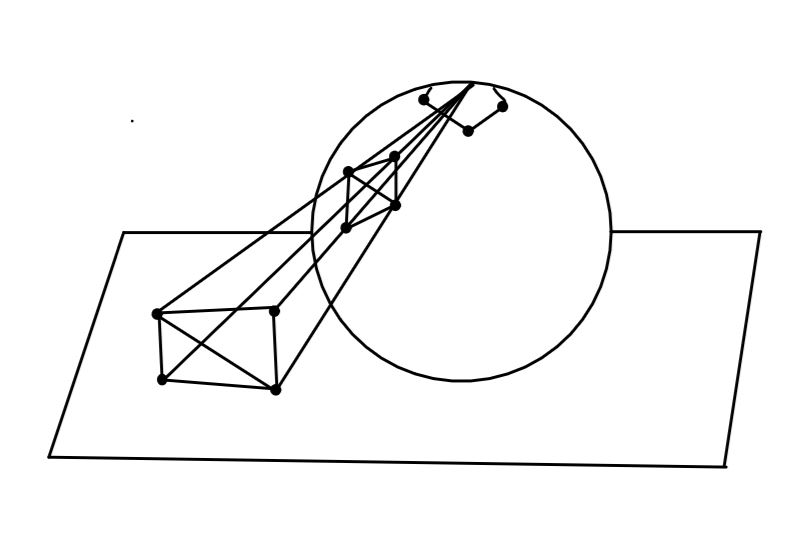
\includegraphics[width=3in]{Images/outerfaceonsphere.JPG}}
\\\\
To invert the unit circle now, or in general any dimensional unit sphere, we use the stereographic map or projection, which is $f(\vec{x})=\dfrac{\vec{x}}{||\vec{x}||^2}$. We can see that any point outside of the unit circle will be mapped inside the circle, because its magnitude is large, and any point in the circle will be mapped out of the circle because its magnitude is less than 1. This works for any point besides the center of the circle, because the magnitude is 0. Then we think of this point becoming the point at infinity when we invert the circle. So a path going to 0 becomes a path going to infinity when we invert the circle.\\
\centerline{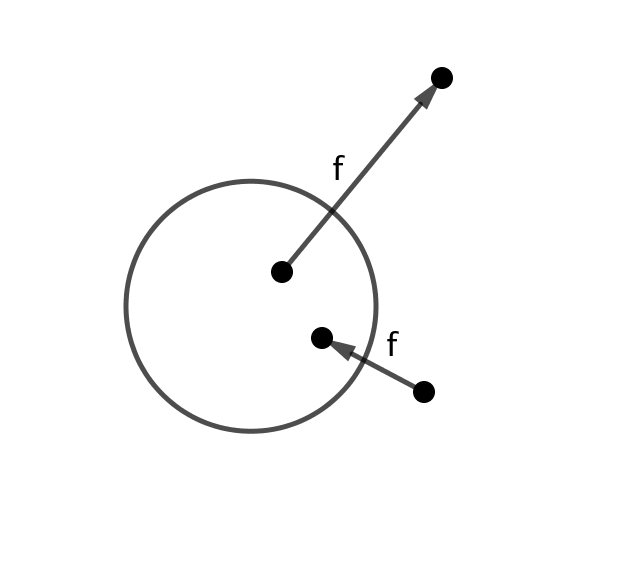
\includegraphics[width=1.75in]{Images/Stereographic.png}}
\\
Then by placing a small hole in the face $F$ (see left figure below) we want to be the outer face, we can invert this circle and all vertices (and other faces) outside $F$ will be projected into $F$, and $F$ will become the outer face (see right figure).
\\
\columnratio{.5,.5}
\begin{paracol}{2}

\begin{leftcolumn}
\centerline{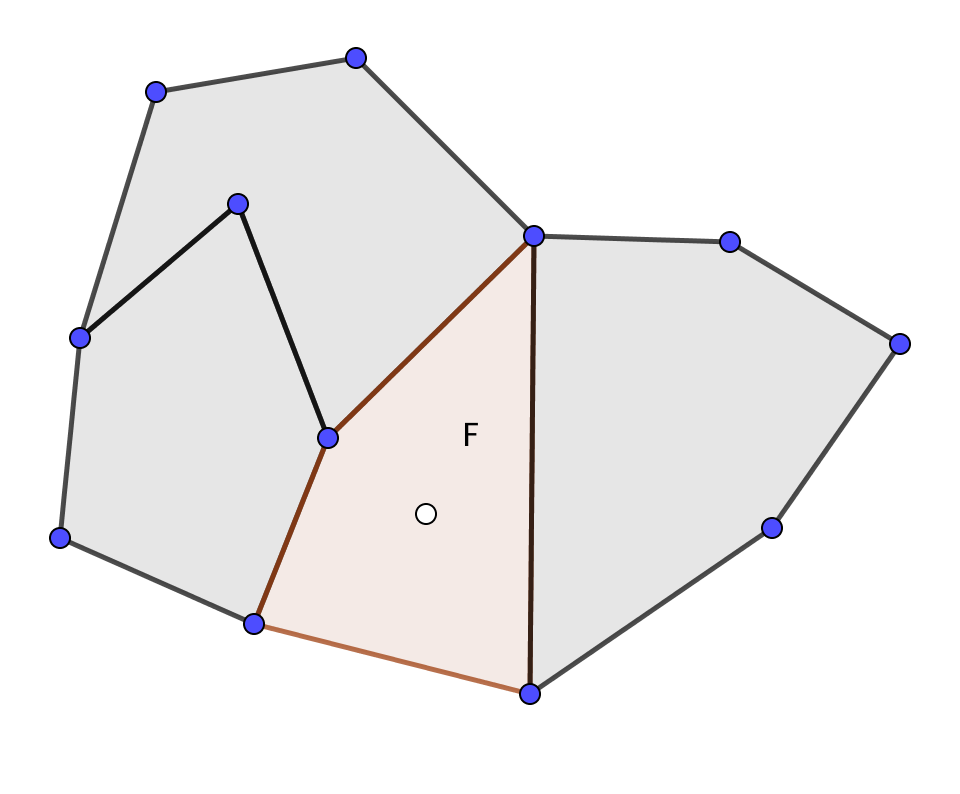
\includegraphics[width=1.75in]{Images/Before.png}}
\end{leftcolumn}
\begin{rightcolumn}
\centerline{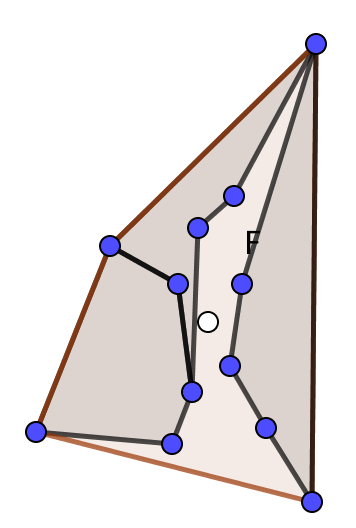
\includegraphics[width=1in]{Images/After.png}}
\end{rightcolumn}
\end{paracol}
\section{Polytopal Graphs}
\begin{definition}
A half-space $H$  is the set of points $(x,y,z)$  such that $ax+by+cz\leq d$, for some $a, b, c, d$.
\end{definition}
\begin{definition}
A polyhedron is the intersection of a finite number of half spaces, i.e. the solutions to $A\vec{x}\leq \vec{b}$.
\end{definition}
\begin{definition}
A polytope is a bounded polyhedron. Equivalently, a polytope is the convex hull of a set of vertices.
\end{definition}
The Fundamental Theorem of Polytopes says that these two definitions are equivalent. Additionally, we are limiting our study to 3 dimensional polytopes. \\\\
We know two things about polytopes currently:
\begin{enumerate}
    \item \textbf{Polytopes are planar.}\\
        If we choose a point outside of the polytope to be a "light source", then illuminating the skeleton of the polytope causes its shadows to form a planar graph. This is a Schlegel diagram, a projection of a polytope from $\mathbb{R}^d$ to $\mathbb{R}^{(d-1)}$ though a point just outside one of its facets. 
    \item \textbf{Polytopes are 3-connected.} \\
    Fact: There always exist monotone paths in every direction. Monotone paths are paths along the edges that always walk in a direction of increasing objective value (for some direction we chose as optimal). This is why the Simplex method works.
    \begin{theorem}
    Polytopes are 3-connected.
    \end{theorem}
    \begin{proof}
    Suppose for contradiction that there exists a cut set $\{x,y\}$. We pick a plane through $x$ and $y$ that separates all vertices either above or below. We call a vertex above the plane $u$ and a vertex below the plane $v$. Then the cross section of the polytope with the plane is a polygon, so we know at least one other edge or vertex passes through the plane. We know there exist monotone paths from $u$ to the northernmost point and from $v$ to the southernmost point. Then, since we know an additional edge passes through the plane, we can find a monotone path from the maximal point to the minimal point through this edge or point, and it does not go through $x$ or $y$ otherwise  it would not be monotone. But if we piece these three paths together, we have a third path from $u$ to $v$. So $\{x, y\}$ was not a cut set and we have a contradiction. Thus, our polytope is 3-connected.
    \end{proof}
\end{enumerate}
\begin{theorem}
For every polytopal graph, there exists an edge we can contract and still get a polytope.
\end{theorem}
\begin{definition}
A simple polytope is a polytope such that if we perturb the half spaces, we still get the same polytope (i.e. vertices, edges and faces).
\end{definition}
Example: Cube\\
Non-Example: Octahedron \\
Note that examples of simple polytopes have degree 3 vertices, because when we increase the degree of a vertex, perturbing the half spaces turns the one vertex into two vertices with an edge between them.



\end{document}

